\section*{Task 1}

\subsection*{Task statement}
Calculate and plot position, velocity, and acceleration trajectories of driving your robot model from configuration $q_0$ to configuration $q_f$ in joint space. 

\subsection*{Solution}

Firstly, to calculate trajectory, we need to find minimum time to reach desired point:

Blending time can be found as:

$$t_b = \frac{\dot q}{\ddot q}$$
where $\dot q$ is maximum velocity and $\ddot q$ is maximum acceleration

Distance travelled during blending:

$$q_b = \frac{\dot q^2}{\ddot q}$$

Distance travelled during non-acceleration phase:

$$q_{na} = |\Delta q| - q_b$$
where $\Delta q = q_f - q_0$

Time of non-acceleration phase:

$$t_{na} = \frac{q_{na}}{\dot q}$$

Then we should check, if $t_{na}$ is negative (or $q_{na}$), then we have enough time to reach the desired point without non-acceleration phase, hence we should use triangular profile, otherwise we should use trapezoidal trajectory

For triangular trajectory:

For this type of trajectory we apply $t_b = \sqrt{\frac{|\Delta q|}{\ddot q}}$

$$
q(t) = 
\begin{cases}
    q_0 + sign(\Delta q) \frac{\ddot q t^2}{2},\ 0 < t \leq t_b \\
    q_0 + sign(\Delta q) (\frac{\ddot q t_b^2}{2} + \ddot q t_b (t - t_b) - \frac{\ddot q (t - t_b)^2}{2}),\ t_b < t \leq t_f
\end{cases}
$$
where $t_f = 2t_b$

For trapezoidal trajectory:

$$
q(t) = 
\begin{cases}
    q_0 + sign(\Delta q) \frac{\ddot q t^2}{2},\ 0 < t \leq t_b \\
    q_0 + sign(\Delta q) (\frac{\ddot q t_b^2}{2} + \dot q (t - t_b)),\ t_b < t \leq t_b + t_{na} \\
    q_0 + sign(\Delta q) (\frac{\ddot q t_b^2}{2} + \dot q t_{na} - \frac{\ddot q (t - t_b - t_{na})^2}{2}),\ t_b + t_{na} < t \leq t_f
\end{cases}
$$
where $t_f = 2t_b + t_{na}$

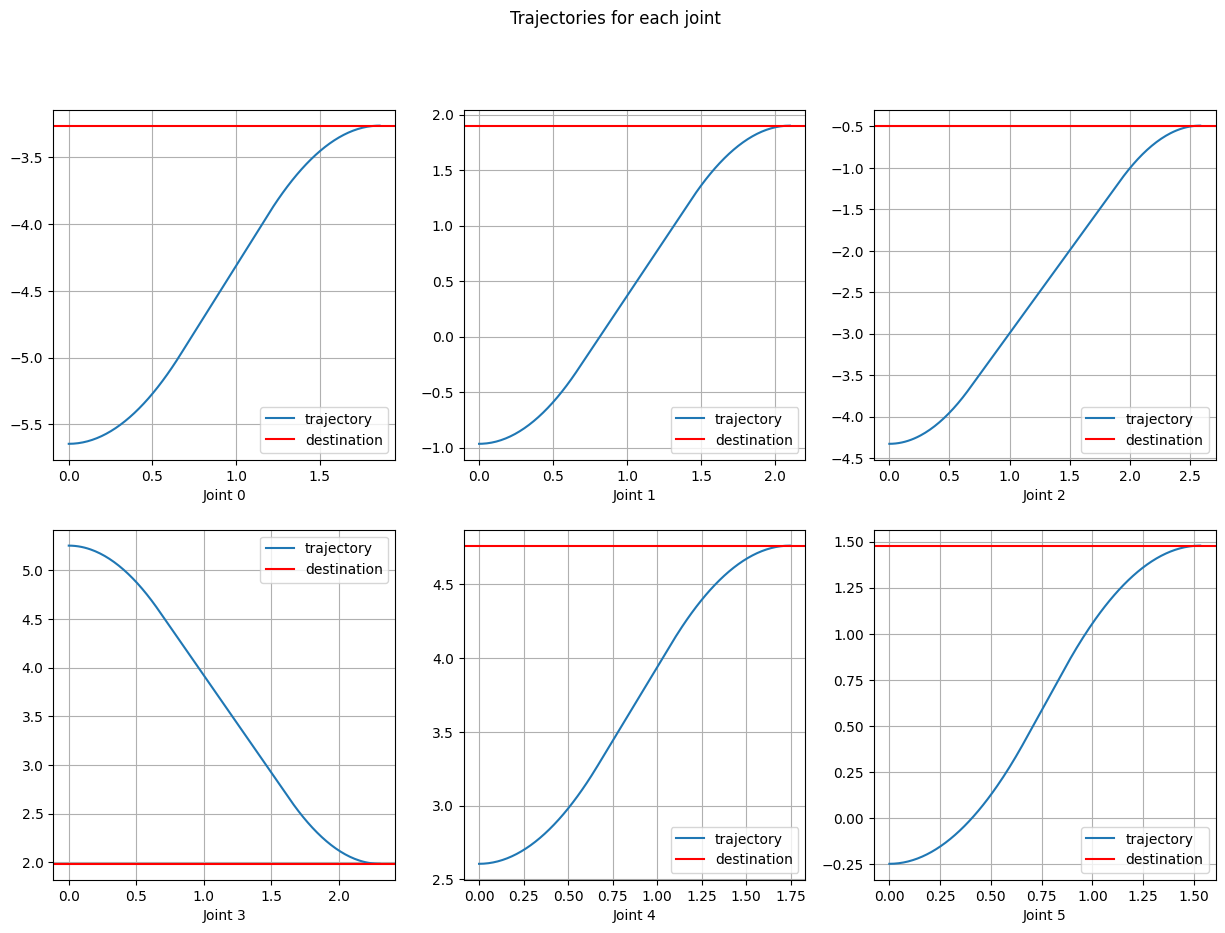
\includegraphics[width=\linewidth]{images/trajectory.png}
